\subsection{Building of the PingaTube}
\label{sec:building-pingatube}

\subsubsection{Materials for the PingaTube}
\label{sec:materials_pingatube}
In order to build the "PingaTube" detector the following parts were used:
\begin{itemize}
\item a cathod consisting in a aluminium tube (l = 146.5 mm, d$_{inner}$ = 20.63
  mm, d$_{outer}$ = 22.9 mm, d$_{window}$ = 9.2 mm)
\item an anode consisting in a Cu/Be wire as the anode (d = 0.025 mm)
\item two brass tubes with the purpose of keeping uniformity on the electric
  field around the anode (d = 1 mm, l$_{1}$ = 40.64 mm and l$_{1}$ = 42.72 mm)
\item insulating endcaps
\item P10 gas Argon (90\%)/CH$_{4}$ (10\%)
\item gas tubes in order to flux the gas (d = 2.1 mm)
\item HV connector in order to supply high voltage to the anode
\item a ground cable in order to connect the cathode.
\item O-ring wire connector
\item electric fastenning belt
\item Ultrasound bath with 10/90 Isopropanol/Water
\item Lab tools (Caliper (precition = 1/100 mm), Needle, Gloves, Files, Drill,
  Saw, Microscope, Oscilloscope, etc) and consumables (Soldering flux, aluminium
  tape, epoxy glue, etc)
\end{itemize}

\subsubsection{Design and Assembly}
\label{sec:design_and_assembly_beercan}
The design was intended for using the aluminium tube as a gas chamber. Most of
the materials were provided and hence creatively assembling the detector was the
main task.  Some pieces were cut by the instructors because of the lab sefety
rules with the mechanical tools. Others such as the brass tubes were prepared by
the students.  Using a lab microscope it was verified that no significant
notches were present on the brass tubes, which was required for the best
functionability possible.  For the assembly of the detector, the parts were
cleaned in an ultrasonic bath of isopropanol/water mixture.

The Cu/Be wire was soldered to the HV connector and glued to the end caps. In
order to fix and seal the chamber the end caps were glued with a two component
epoxy glue.  The Cu/Be wire was inserted thru two brass tubes in both the
extremes of the chamber in order to ensure as uniform field as possible.  A
window in a form of circular hole was drilled around the middle part of the
chamber. The end caps have holes to provide access for gas tubes, they were
glued in both sides with the epoxy glue.  The Cu/Be wire and the pipe were
connected and soldered the high voltage connector as anode and ground
respectively. A part of the aluminum tube was polished to create space for
grounding and that surface was covered with copper tape for providing better
contact.  Given that the Cu/Be is toxic gloves were required for handling it.
Additionally the wire easily bends increasing the risk of it being break. The
wire was soldered to the extremes of the brass tubes already mounted in the end
caps. All was sealed with the epoxy glue afterwards.

After the assembly process the P10 gas was flushed into the detector in order to
extract as much O$_2$ as possible. The main reason of this is O$_2$ is a
quenching gas that absorbs the avalanche electrons.  Presence of leakages of gas
from the detector tube was checked with a flowmeter.

Volume of the aluminum tube: \emph{Volume of the tube}, Volume of the tube
\begin{equation}
  \label{eq:tube_volume}
  V=\frac{\pi L^2}{4} =14.65*3.14*2.06324*2.06324=48,96 cm^3
\end{equation}
With a flow 10 ml/min = 600 cm$^3$/h content of the volume changes ~10 times per
hour. The variation of O$_{2}$ concentration with time is shown on
Figure~\ref{fig:}. Units of x-axis are ppm = 1,000,000 m$_{c}$ / m$_{s}$, where
m$_{c}$ = mass of component (argon/methane mix, kg) m$_{s}$ = mass of solution
(oxygen, kg)

Some failures which were fixed were:
\begin{itemize}
\item one of the gas tubes did were not interted properly which caused gas
  leaking, The problem was sucessfuly fixed afterwards by removing and
  reinserting it properly.  This caused a lot of delay due to the time that the
  glue delays on drying besides the fact that it was needed to reflux the gas on
  the detector.
\item There were some gas leakages that were sorted out propperly by glue
  sealing the positions in which the floweter detector establish the gas
  leakages.
\item One of the brass tubes went loose inside of the aluminium tube. The issue
  was sorted out on time before the glu dried without any further problem.
\end{itemize}

\subsection{Building of the "BeerCan" detector}
\label{sec:building_beercan}

\subsubsection{Materials for the BeerCan}
\label{sec:materials_beercan}
In order to build the "BeerCan" detector the following parts were used:
\begin{itemize}
\item a catode consisting in a beer can (l = 146.5 mm, d$_{inner}$ = 64.0 mm,
  d$_{thickness}$ = 0.2 mm)
\item an anode consisting in a Cu/Be wire as the anode (d = 0.025 mm)
\item two brass tubes. (d = 1 mm, l$_{1}$ = 40.64 mm and l$_{1}$ = 42.72 mm)
\item guide in order to protect the brass tubes of touching the can (d = 3.21
  mm)
\item bushing
\item plastic endcaps
\item gas tubes in order to flux the gas (d = 2.1 mm)
\item HV connector in order to supply high voltage to the anode
\item a ground cable in order to connect the cathode.
\item P10 gas Argon (90\%)/CH$_{4}$ (10\%)
\item Ultrasound bath with 10/90 Isopropanol/Water
\item Lab tools (Caliper (precition = 1/100 mm), Needle, Gloves, Files, Drill,
  Saw, Microscope, Oscilloscope, etc) and consumables (Soldering flux, aluminium
  tape, epoxy glue, etc)
\end{itemize}

\subsubsection{Design and Assembly of the BeerCan}
\label{sec:design_and_assembly_beercan}
The design was intended for using a beer can as gas chamber detector. The
building and assembly was very similar to the description on the PingaTube
detector with the mechanical differences imposed by the beer can geometry.
Again most of the materials were provided and hence creatively assembling the
detector was the main task. After the assembly process the P10 gas was flushed
into the detector and the flowmeter was used for detecting gas leakages.

Volume of the beercan tube:
\emph{Volume of the tube}, Volume of the tube
\begin{equation}
  \label{eq:tube_volume}
  V=\frac{\pi L^2}{4} =14.65*3.14*6.40*6.40=471,05 cm^3
\end{equation}
With a flow 10 ml/min = 600 cm$^3$/h content of the volume changes ~10 times per
hour.  The variation of O$_{2}$ concentration with time is shown on Fig.Units of
x-axis are ppm = 1,000,000 m$_{c}$ / m$_{s}$, where m$_{c}$ = mass of component
(argon/methane mix, kg) m$_{s}$ = mass of solution (oxygen, kg)

Some failures:
\begin{itemize}
\item There was gas leaking in the endcaps, they were sealed by using the epoxy
  gum and covering all the leaking points detected.
  \item The Cu/Be wire got blended and a little bit loose while trying to solder
    it to the one of the brass tubes which might have cause the detector to have
    an extremely poor signal hence it was considered a failure. There was not
    enough time for fixing this issue since it practically would have taken the
    dissasembly of the whole detector.
\end{itemize}

\subsection{Measurement apparatus}
\label{sec:meas-appar}
Figure~\ref{fig:exp_setup} shows a schematic view of the setup used for the
calibration of the detector and data taking. The signal from the detector at
first pass trough a pre-amplifier, this has a capacitance of 1~pF and is
connected to a high voltage (HV) power supply so that the input voltage is
directly proportional to the charge generated in the detector through the well
know formula\autocite{Knoll:RadMeasurement}
\begin{equation}
  \label{eq:capacitance}
  Q = CV.
\end{equation}
The pre-amplifier is then connected to a spectrum amplifier with adjustable gain
and a pulse generator. From the spectrum amplifier the signal was sent to an
oscilloscope for online monitoring and adjustments and to a multi-channel
analyzer (MCA) that was connected to a computer to record the data.
\begin{figure}[!h]
  \centering
  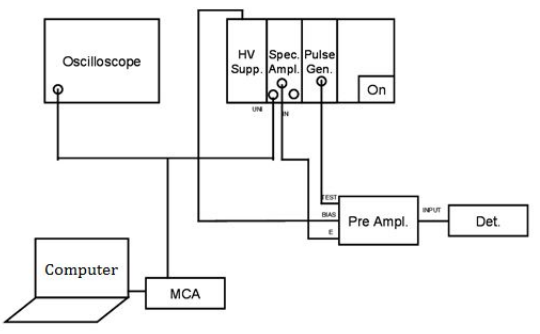
\includegraphics[width=.5\linewidth]{experimental_setup}
  \caption{Schema of the experimental setup}
  \label{fig:exp_setup}
\end{figure}
%%% Local Variables:
%%% mode: latex
%%% TeX-master: "prop_counter"
%%% End:
